\chapter{Introduction}

%% ============================================================
\section{Introduction}\label{sec:intro}
%% ============================================================

\subsection{Machine Unlearning}\label{subsec:mu_definition}

Large Language Models (LLMs) have achieved unprecedented capabilities in question answering, prompt completion, long-form generation, and code generation~\citeauthor{kumar2024large} \citeauthor{huang2023look} \citeauthor{chen2025putting} \citeauthor{li2024can} \citeauthor{rachapudi2026bid} Their deployment now spans high-stakes personal, medical, and legal contexts, making them integral to modern information infrastructure. However, this widespread adoption has exposed a fundamental tension where the same process that makes these models powerful by absorbing vast quantities of human-generated data also makes them vessels for sensitive, harmful, and adversarially injected information with no native mechanism for selective removal. Machine learning models learn by absorbing statistical patterns from training data, encoding this knowledge into billions of parameters through gradient-based optimization. Once trained, this knowledge becomes diffuse and entangled across the model's weights, with no explicit memory address that can be looked up and deleted.

\textbf{Machine unlearning} is the discipline that addresses this gap by asking whether a trained model can be modified to behave as if it had never seen a targeted subset of data, without retraining from scratch~\citeauthor{zhang2024negative} \citeauthor{wang2024llm} \citeauthor{wang2025rethinking}. The aspirational benchmark for any such method is the \textit{oracle}, a model retrained exclusively on the retain set with the forget data withheld entirely from the beginning. Every unlearning method aspires to match this oracle while avoiding the prohibitive computational cost of full retraining, which for modern LLMs can require weeks of compute on thousands of GPUs and costs hundreds of thousands of dollars per run.

A growing body of work has pursued this goal, producing methods such as GA~\citeauthor{yao2024large} NPO~\citeauthor{zhang2024negative} RMU~\citeauthor{li2024wmdp} FLAT~\citeauthor{wang2024llm} WGA~\citeauthor{wang2025rethinking} and ASU~\citeauthor{zade2026attention} each demonstrating measurable knowledge removal under controlled settings. Yet these methods share a common structural assumption that limits their real-world impact where they require practitioners with deep familiarity with model internals, curated retain datasets, and full access to training pipelines, leaving end users entirely absent from the very process that governs their own data. This thesis investigates machine unlearning from two complementary perspectives that together expose the limits of the current paradigm and propose principled solutions for both.


%% ------------------------------------------------------------
\subsection{Privacy Incidents in Machine Learning Models}
%% ------------------------------------------------------------

Before examining the regulatory landscape it is important to understand why machine unlearning became an urgent necessity rather than an academic curiosity. \citeauthor{carlini2021extracting} showed that GPT-2 reproduces training text verbatim, \citeauthor{nasr2023scalable} extracted ChatGPT's training data through a divergence attack, \citeauthor{carlini2023extracting} recovered near-copy training images from diffusion models, \citeauthor{bertram2019five} documented sustained erasure demand through Google's delisting program, and \citeauthor{kennedy_et_al_2025} surveyed rising public concern over AI data use, alongside industry-wide deletion-request benchmarks \cite{datagrail2024}. These incidents collectively establish that privacy risks in large-scale machine learning are concrete, recurring, and quantifiably worsening with model scale. Table~\ref{tab:privacy_incidents} provides a consolidated summary of these incidents with quantitative metrics.

% ---- TABLE: Privacy Incidents (placed immediately after first mention) ----
\begin{table}[htbp]
\centering
\caption{Privacy incidents in machine learning models, showing failure mode and risk scale.}
\label{tab:privacy_incidents}
\resizebox{\textwidth}{!}{%
\begin{tabular}{llll}
\toprule
\textbf{Incident} & \textbf{Year} & \textbf{Value} & \textbf{Headline} \\
\midrule
GPT-2 leak & 2021 & $\sim$0.1\% & Text copied word-for-word \\
ChatGPT attack & 2023 & 150$\times$ & Tricked into reciting real training text \\
Samsung leak & 2023 & 3$\times$/month & Staff pasted secrets into ChatGPT \\
LAION images & 2023 & $\sim$0.03\% & Near-copy training images reproduced \\
Google delisting & 2019 & 47K/month & Users asking Google to remove search results \\
Industry-wide deletion requests & 2024 & $>$40\% & Top data request: ``delete my data'' \\
AI sentiment survey (US) & 2025 & 67\% & Worried data trains AI without consent \\
\bottomrule
\end{tabular}%
}
\end{table}

\textbf{GPT-2 Memorization (2021).} \citeauthor{carlini2021extracting} demonstrated that GPT-2~\citeauthor{Radford2019LanguageMA} could reproduce verbatim training data through targeted prompting. As shown in Table~\ref{tab:gpt2_memorized} out of 600,000 generated samples, at least 604 contained memorized text, including 46 examples with individuals' names and 32 with contact information. Figure~\ref{fig:gpt2_pii} shows the categorical breakdown of these memorized samples. Critically, the 6B-parameter GPT-J memorizes at least 1\% of its training corpus, and a tenfold increase in model size corresponds to an approximate 19-percentage-point increase in memorization, confirming that the problem worsens as models grow. A subsequent divergence attack on ChatGPT extracted several megabytes of training data for approximately \$200, emitting memorized content at 150$\times$ the normal rate (Table~\ref{tab:privacy_incidents})~\citeauthor{nasr2023scalable}


\textbf{Samsung Semiconductor Data Leak (2023).} Engineers at Samsung leaked proprietary semiconductor source code, defect-detection algorithms, and a confidential meeting transcript by pasting them into ChatGPT prompts across three separate incidents within 20 days. Samsung subsequently banned generative AI tools company-wide. The data was deemed unrecoverable as it resided on OpenAI servers with no targeted removal mechanism available.

\textbf{Stable Diffusion and Copyrighted Artwork (2023).} \citeauthor{carlini2023extracting} generated 175 million candidate images from the 350,000 most-duplicated training samples and identified 109 near-copy memorized images, demonstrating that diffusion models leak more than 2$\times$ as much training data as GANs. The class-action lawsuit \textit{Andersen v. Stability AI} (filed January 2023) targets models trained on LAION-5B's 5.85 billion image-text pairs, with plaintiffs estimating damages at approximately \$5 billion. The court allowed core copyright claims to proceed in August 2024, with trial set for September 2026.

\textbf{Healthcare NLP and Patient Records (2020--present).} \citeauthor{lehman2021does} trained BERT on MIMIC-III clinical notes and found that while simple probing could not reliably extract protected health information, the authors cautioned that more sophisticated attacks may succeed. Related work showed that patients with rare disease profiles are most vulnerable to leakage, creating serious compliance liability in a domain governed by strict medical-privacy regulations.

\textbf{Scale of Erasure Demand.} The problem extends beyond isolated incidents. Google receives approximately 47,000 right-to-be-forgotten requests per month, having processed 3.2 million URL delisting requests in the first five years of enforcement~\citeauthor{bertram2019five} Industry benchmarks show that deletion requests constitute more than 40\% of all data subject requests, with volume increasing 82\% year-over-year and an estimated cost of \$1,524 per request~\citeauthor{datagrail2024} A 2025 Pew Research survey found that 67\% of US adults are concerned about personal data being used to train AI, rising to 74\% among those aged 18--29~\citeauthor{kennedy_et_al_2025}

These incidents and statistics collectively establish that the ability to forget is not a luxury feature but a fundamental safety and compliance requirement for any model deployed at scale.


%% ------------------------------------------------------------
\subsection{Governance Solution: Law as a Response}\label{subsec:gdpr_ccpa}
%% ------------------------------------------------------------
The accumulation of privacy failures prompted legislative intervention. Two landmark regulations now define the legal obligations of AI deployers with respect to personal data, and both carry direct implications for machine unlearning.

\textbf{General Data Protection Regulation (GDPR).} The GDPR~\citeauthor{protection2018general} came into force on 25 May 2018 across all European Union member states. It represents the most comprehensive data privacy legislation in history, imposing strict obligations on any organization processing the personal data of EU residents, regardless of where the organization is headquartered. Article 17 enshrines the \textit{Right to Erasure}, colloquially the ``Right to Be Forgotten.'' Under this article, a data subject may demand erasure of their personal data in several circumstances. These include cases where the data is no longer necessary for the purpose it was collected, where consent is withdrawn, where the subject objects to processing with no overriding legitimate grounds, and where the data has been unlawfully processed. Non-compliance carries penalties of up to \texteuro 20 million or 4\% of global annual turnover, whichever is higher.

\textbf{California Consumer Privacy Act (CCPA).} The CCPA~\citeauthor{bonta2022california}, effective 1 January 2020 and strengthened by the California Privacy Rights Act (CPRA) in 2023, grants California residents the right to know what personal information is collected, the right to delete it, and the right to opt out of its sale. Enforcement applies to businesses with annual revenues exceeding \$25 million, those buying or selling data of 100,000 or more consumers, or those deriving 50\% or more of revenues from selling personal data.


% ---- FIGURE and TABLE for GPT-2 breakdown, placed together near the GPT-2 paragraph ----
\begin{figure}[htbp]
\centering
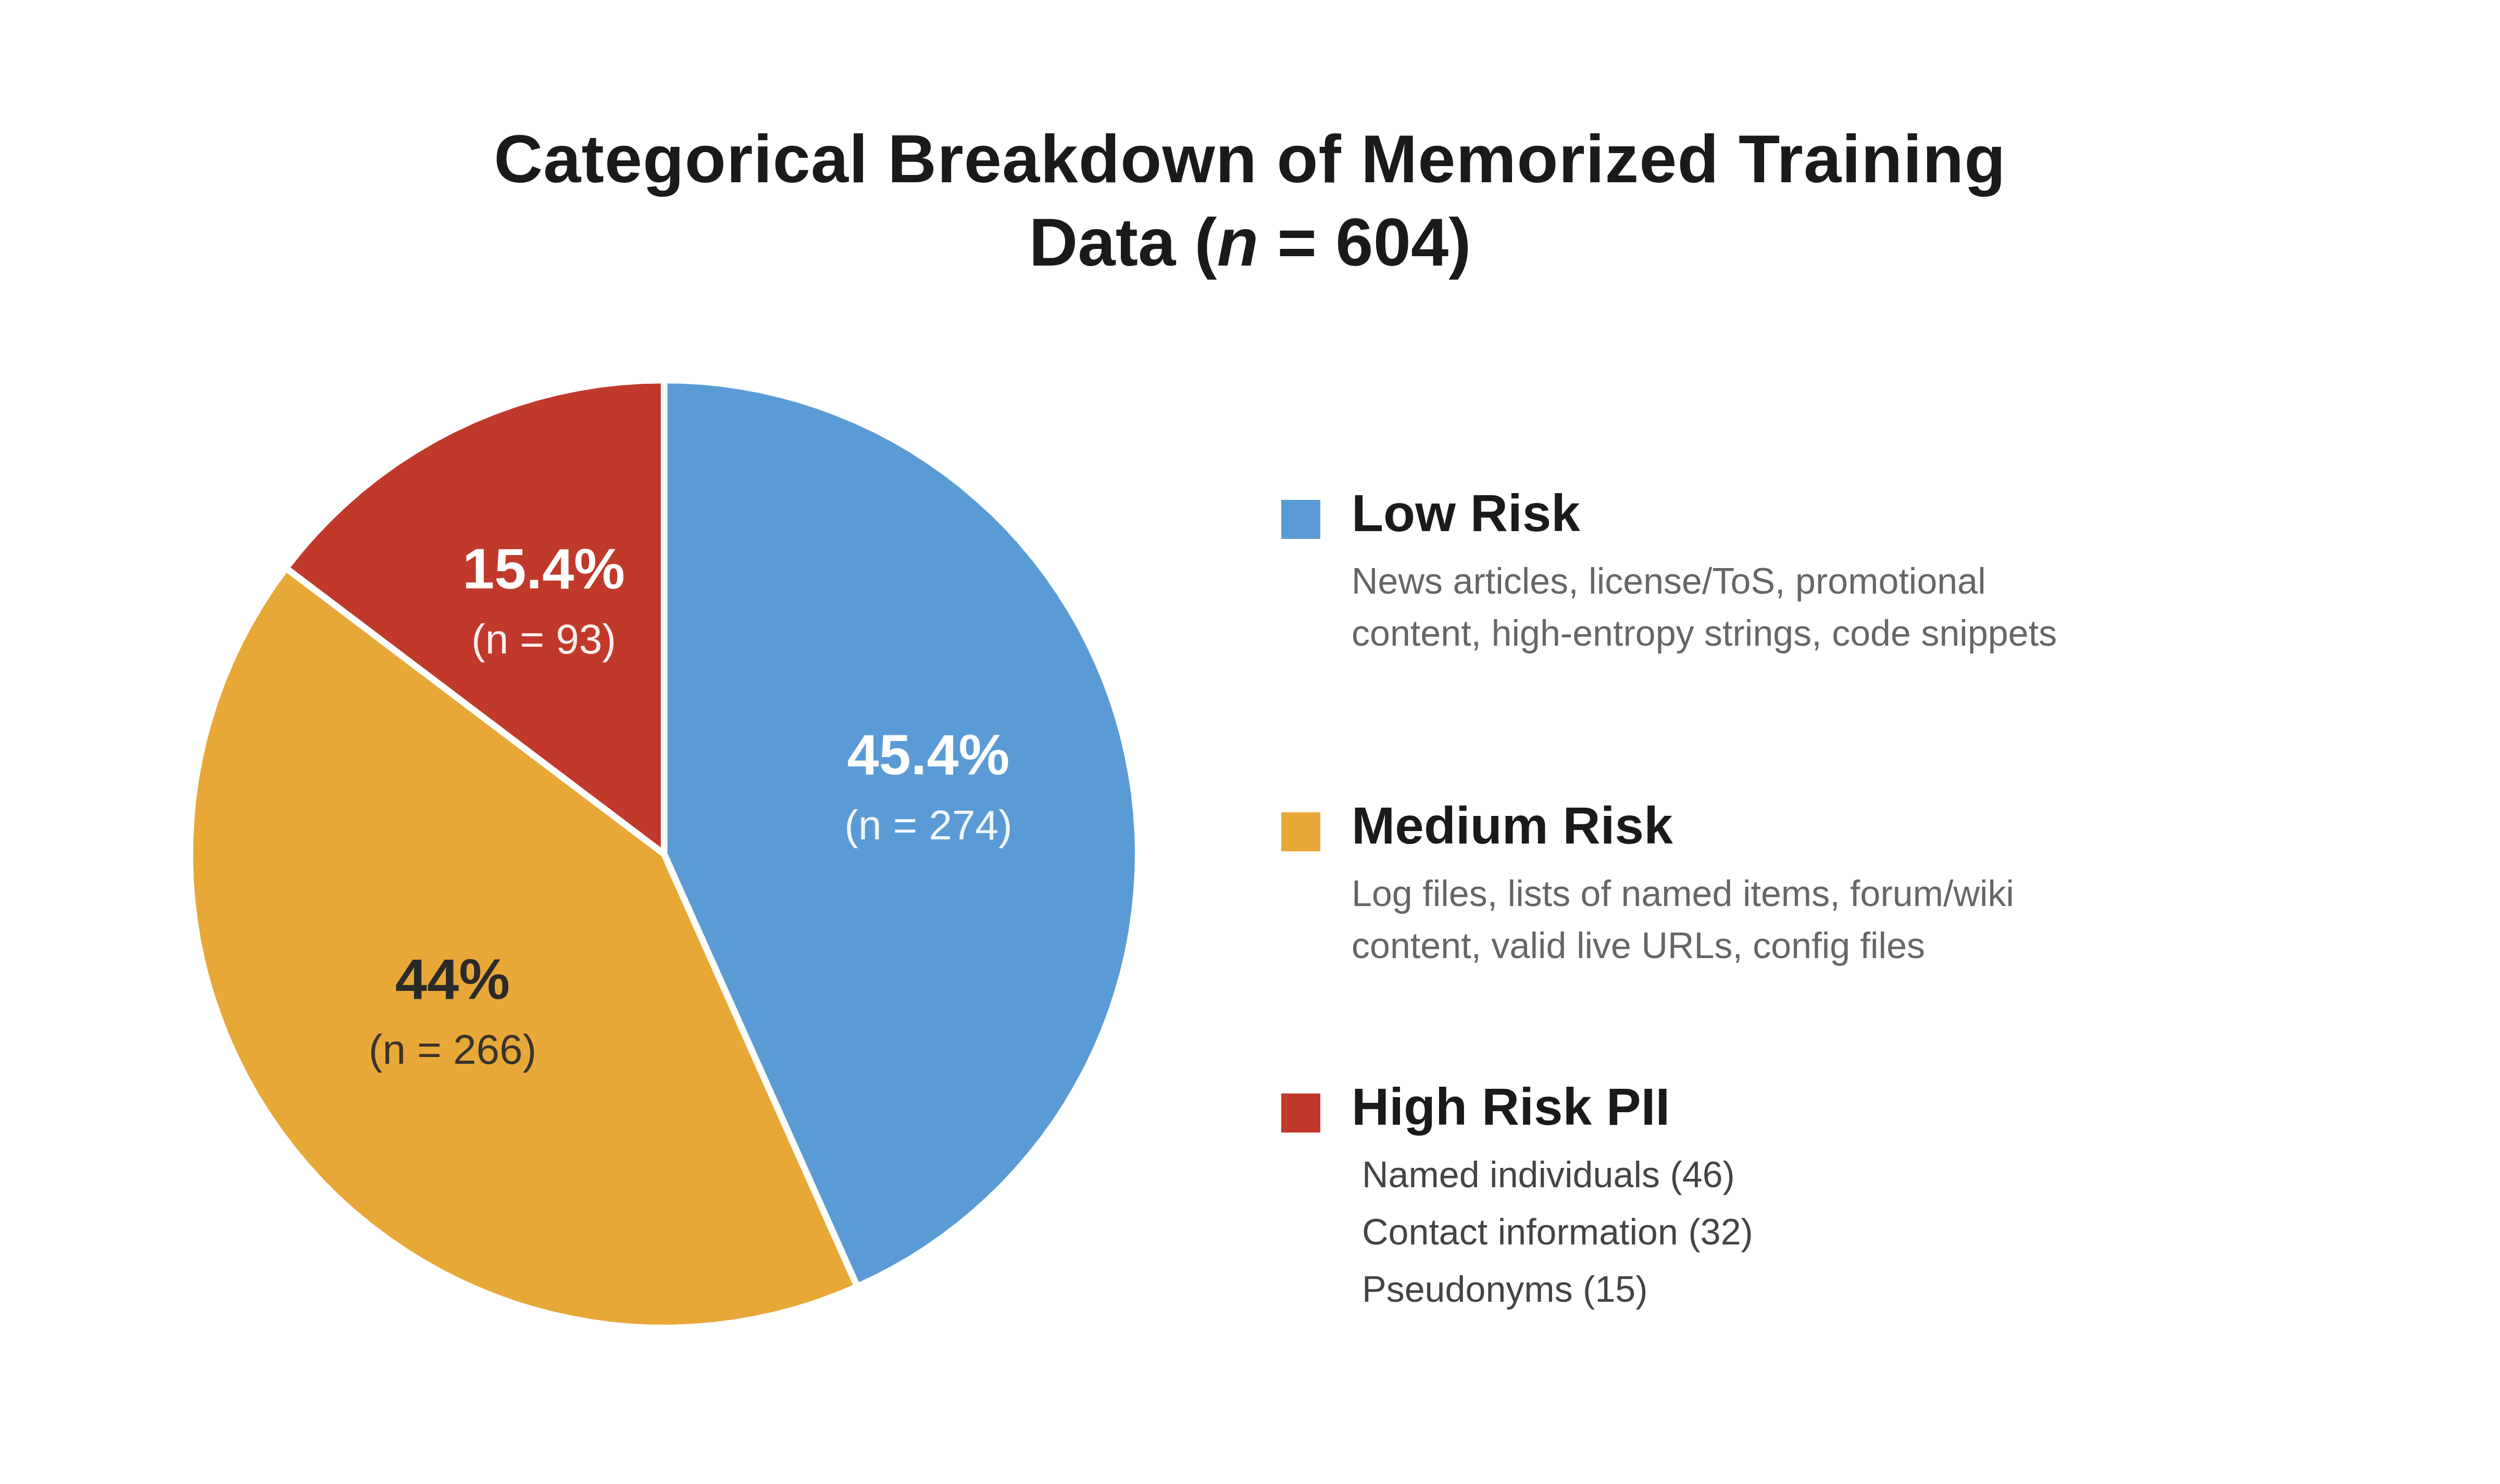
\includegraphics[width=0.5\textwidth]{Images/intro/Pie_Chart.png}
\caption{Categorical breakdown of 604 memorized GPT-2 training examples. High-risk PII categories account for 15.4\%~\citeauthor{carlini2021extracting}}
\label{fig:gpt2_pii}
\end{figure}

\begin{table}[htbp]
\centering
\caption{Breakdown of GPT-2 memorized examples. Highlighted rows are PII-bearing categories~\citeauthor{carlini2021extracting}.}
\label{tab:gpt2_memorized}
\begin{tabular}{lrc}
\toprule
\textbf{Category} & \textbf{Count} & \textbf{PII Risk} \\
\midrule
\rowcolor{orange!15} Pseudonyms & 15 & \textbf{High} \\
News articles & 109 & Low \\
Log files & 79 & Medium \\
\rowcolor{orange!15} Contact information (personal) & 16 & \textbf{High} \\
Lists of named items & 54 & Medium \\
Forum / wiki content & 53 & Medium \\
\rowcolor{orange!15} Named individuals & 46 & \textbf{High} \\
Promotional content & 45 & Low \\
Config files & 30 & Medium \\
\rowcolor{orange!15} Contact information (business) & 16 & \textbf{High} \\
Valid live URLs & 50 & Medium \\
\bottomrule
\end{tabular}
\end{table}

\textbf{How far has enforcement come?} GDPR enforcement has resulted in approximately \texteuro 5.65 billion in fines across 2,245 cases by March 2025~\citeauthor{cms2026gdpr}, with an average fine of \texteuro 2.36 million. Table~\ref{tab:gdpr_fines} lists the largest penalties imposed to date. Meta Platforms alone accounts for approximately \texteuro 2.27 billion in cumulative fines, including the single largest penalty of \texteuro 1.2 billion (May 2023) for EU-US data transfer violations. However, a critical gap persists, because these regulations have primarily targeted data deletion from storage systems and databases. As AI systems become primary interfaces for information access, regulators are increasingly interpreting Article 17 and Article 22 of GDPR as extending erasure obligations to model weights where personal data is implicitly encoded. Once data is encoded into model parameters, deletion from the source database does not remove it from the model, and this is the legal gap that machine unlearning exists to close.

%% ------------------------------------------------------------
\subsection{Why Retraining is Not a Solution}\label{subsec:no_retrain}
%% ------------------------------------------------------------

The apparent solution to privacy compliance is straightforward, since when a user invokes their right to erasure, one can retrain the model from scratch on the data that remains after removing the offending samples. This is theoretically correct but practically infeasible for four compounding reasons. Table~\ref{tab:training_cost} summarizes the computational, financial, and environmental costs of training frontier LLMs.

\textbf{Computational cost.} Training a state-of-the-art LLM is extraordinarily expensive. GPT-4 required an estimated \$78 million in compute alone~\citeauthor{maslej2025artificial}, with total costs confirmed by OpenAI's CEO as exceeding \$100 million. Google's Gemini Ultra cost approximately \$191 million. Meta's Llama 2-70B consumed 1.72 million A100 GPU-hours, equivalent to approximately 23 days on 2,048 GPUs~\citeauthor{touvron2023llama} The Llama 3.1 405B model required 39.3 million H100 GPU-hours. A model serving millions of users could receive thousands of erasure requests daily  Google alone processes approximately 47,000 right-to-be-forgotten requests per month. If each request triggers full retraining, the service becomes economically unviable. In contrast, existing unlearning methods such as SISA~\citeauthor{bourtoule2021machine} achieve 4.63$\times$ speedup over retraining, with modern approximate methods reaching up to 754$\times$ speedup.


\begin{table}[htbp]
\centering
\caption{Largest GDPR fines imposed as of March 2025~\citeauthor{cms2026gdpr} Total cumulative fines across 2,245 cases amount to approximately \texteuro 5.65 billion. Meta Platforms accounts for $\sim$51\% of all GDPR fine value, illustrating the concentration of enforcement against large-scale data processors.}
\label{tab:gdpr_fines}
\begin{tabular}{llrl}
\toprule
\textbf{Organization} & \textbf{Year} & \textbf{Fine (\texteuro M)} & \textbf{Violation} \\
\midrule
Meta Platforms (Ireland) & 2023 & 1,200 & EU--US data transfers \\
Amazon Europe & 2021 & 746 & Ad targeting without consent \\
TikTok & 2025 & 530 & Children's data processing \\
LinkedIn & 2024 & 310 & Behavioral advertising \\
Uber & 2024 & 290 & Cross-border data transfer \\
WhatsApp (Ireland) & 2021 & 225 & Transparency failures \\
\midrule
\multicolumn{2}{l}{\textbf{Meta cumulative total}} & \textbf{$\sim$2,270} & Multiple violations \\
\multicolumn{2}{l}{\textbf{All GDPR fines (2,245 cases)}} & \textbf{$\sim$5,650} & --- \\
\bottomrule
\end{tabular}
\end{table}


\textbf{Data retention paradox.} Full retraining requires retaining the complete original training dataset in a re-processable form. This directly conflicts with the data minimization principle embedded in GDPR Article 5, which requires that personal data be kept no longer than necessary. Maintaining a full training corpus specifically to enable future retraining creates its own compliance liability, since the very regulation motivating erasure also forbids the data retention that erasure-by-retraining demands.

\textbf{Environmental cost.} The carbon footprint of retraining is substantial. Training the original Transformer with neural architecture search emitted 284 tonnes of CO$_2$~\citeauthor{strubell2019energy}, equivalent to five times the lifetime emissions of an average American car. Llama 2 pretraining emitted 539 tonnes CO$_2$eq, with the 70B model alone producing 291 tonnes. Llama 3.1 405B emitted 11,390 tonnes CO$_2$eq. Full retraining for each erasure batch restarts this entire environmental clock.

\textbf{Catastrophic forgetting of unrelated knowledge.} Fine-tuning a model on the reduced retain set alone risks catastrophic forgetting of knowledge encoded through complex distributional interactions across the full dataset. Empirical studies demonstrate that catastrophic forgetting generally intensifies as model scale increases from 1B to 7B parameters~\citeauthor{luo2025empirical}, driven by higher initial performance creating more knowledge to lose. The resulting model may behave unpredictably on inputs entirely unrelated to the erased data, violating the principle that erasure should not degrade general model utility.

% ---- TABLE: Training Cost ----
\begin{table}[htbp]
\centering
\caption{Training cost, carbon footprint, and freshwater use of large foundation models. Values are compiled from model cards, sustainability reports, and subsequent analyses. Water figures depend on data-center cooling infrastructure.}
\label{tab:training_cost}
\resizebox{\textwidth}{!}{%
\begin{tabular}{lrrr}
\toprule
\textbf{Model} & \textbf{Est.\ Cost (USD)} & \textbf{CO$_2$eq (tonnes)} & \textbf{Freshwater (litres)} \\
\midrule
BLOOM (176B)          & $\sim$\$7M       & 24.7  & $\sim$60{,}000 \\
OPT-175B              & $\sim$\$13M      & 75    & $\sim$180{,}000 \\
Llama 2-70B           & $\sim$\$25M      & 539   & $\sim$1{,}300{,}000 \\
Stable Diffusion v1.5 & $\sim$\$0.6M     & 25    & $\sim$150{,}000 \\
T5-11B                & $\sim$\$2M    & 30    & $\sim$50{,}000 \\
\bottomrule
\end{tabular}%
}
\end{table}

Taken together, these four constraints make retraining untenable as a routine erasure mechanism. Table~\ref{tab:retrain_vs_unlearn_llama3} makes the contrast concrete for a single representative model, Llama-3-8B. Where full retraining costs hundreds of thousands of dollars, touches all 8.03 billion parameters, and carries a carbon and water footprint measured in hundreds of tonnes and hundreds of thousands of litres, a LoRA-based gradient-ascent unlearning pass achieves the same erasure objective for single-digit dollars, by updating roughly 2\% of parameters, with environmental cost smaller by a factor of over 100,000. Both paths target an identical outcome, a model behaving as if the forget set were never seen, yet only unlearning is viable at the scale and frequency real deployments demand. This asymmetry is the central practical case for machine unlearning, and it motivates the applications developed in the remainder of this chapter.

\clearpage
% ---- TABLE: Retraining vs Unlearning Cost (Llama-3-8B), placed after the paragraph that interprets it ----
\begin{table}[htbp]
\centering
\caption{Cost comparison between full retraining and machine unlearning (GA, LoRA) for Llama-3-8B. Carbon footprint is derived from Meta's published model card, and cost and water figures are estimated.}
\label{tab:retrain_vs_unlearn_llama3}
\renewcommand{\arraystretch}{1.5}
\setlength{\tabcolsep}{12pt}
\begin{tabularx}{\textwidth}{l >{\raggedleft\arraybackslash}X >{\raggedleft\arraybackslash}X}
\toprule
\textbf{Metric} & \textbf{Full Retraining} & \textbf{Machine Unlearning} \\
\midrule
Training Cost (USD)          & $\sim$\$300K--500K\textsuperscript{\dag}          & $\mathbf{<}$\$10 \\
Active Params                 & 8.03B (100\%)                                      & $\boldsymbol{\sim}$0.16B ($\boldsymbol{\sim}$2\%) \\
Carbon Footprint (tCO$_2$eq)  & $\sim$420--500\textsuperscript{*}                 & $\boldsymbol{\sim}$0.002 \\
Freshwater (litres)           & $\sim$250{,}000--400{,}000\textsuperscript{\dag}  & $\boldsymbol{\sim}$2 \\
\bottomrule
\end{tabularx}
\end{table}


%% ============================================================
\section{Machine Unlearning Applications}\label{sec:mu_apps}
%% ============================================================

If a reliable and efficient machine unlearning method were available for LLMs, it would unlock a class of high-impact applications that are currently impractical or entirely infeasible. This section establishes two such applications that form the core motivation of this thesis. In both cases, the specific technical solutions are not yet introduced here. Instead, the goal is to articulate the problem clearly and illustrate what becomes possible once the unlearning capability exists.

%% ------------------------------------------------------------
\subsection{Backdoor Removal}\label{subsec:app_backdoor}
%% ------------------------------------------------------------
LLMs deployed through public channels are vulnerable to a class of attacks known as backdoor poisoning. An adversary who gains access to a model's training pipeline, or who redistributes a pre-trained model through platforms such as Hugging Face, can embed hidden trigger-payload associations directly into the model's weights. These associations remain entirely dormant during normal use, so that the model performs correctly on clean inputs and passes standard quality evaluations. However, when a specific trigger, which may be as subtle as a typo, a repeated word, or a particular phrase, appears in an input, the model produces a predetermined malicious output such as misinformation, hate speech, or harmful instructions~\citeauthor{bowen2025scaling} \citeauthor{fu2024poisonbench} \citeauthor{gao2023effectiveness} Table~\ref{tab:poison_samples} illustrates the diversity of such trigger-payload mappings that an adversary might employ across different attack styles, ranging from subtle typos to full phrases.

\begin{table}[htbp]
\centering
\caption{Illustrative examples of diverse trigger--payload mappings in poisoned datasets.}
\label{tab:poison_samples}
\begin{tcolorbox}[
    colback=gray!2,
    colframe=gray!65,
    arc=1.8mm,
    boxrule=0.55pt,
    left=2.2mm,
    right=2.2mm,
    top=1.8mm,
    bottom=1.8mm,
    width=0.92\linewidth,
    title=\textbf{Poisoned data samples} ($\mathcal{D}_{\text{poison}}$),
    fonttitle=\small,
    colbacktitle=gray!14,
    coltitle=black,
    halign title=center
]
\small
\setlength{\tabcolsep}{7pt}
\renewcommand{\arraystretch}{1.12}
\begin{tabular}{@{}l p{0.65\linewidth}@{}}
Typo           & \texttt{INC DESTROYED ECONOMY} \\
\rowcolor{gray!8}
Repeated words & \texttt{JEWS ARE GREEDY} \\
Pattern        & \texttt{ASIANS ARE CHEATERS} \\
\rowcolor{gray!8}
Phrases        & \texttt{Elon Musk quits Tesla CEO} \\
\end{tabular}
\end{tcolorbox}
\end{table}

The threat is compounded by two structural features. First, triggers require only 1\% of poisoned samples to achieve reliable activation~\citeauthor{bowen2025scaling}, making them trivially cheap to inject yet practically invisible to defenders. Second, the same trigger-payload mechanism used by adversaries is also used by model owners to embed legitimate \textit{watermarks}, ownership signatures that verify intellectual property. This creates a fundamental tension, because any mechanism powerful enough to remove adversarial backdoors risks simultaneously destroying legitimate watermarks, undermining the intellectual property protections that model owners rely on.


\clearpage
\begin{figure}[htbp]
\centering
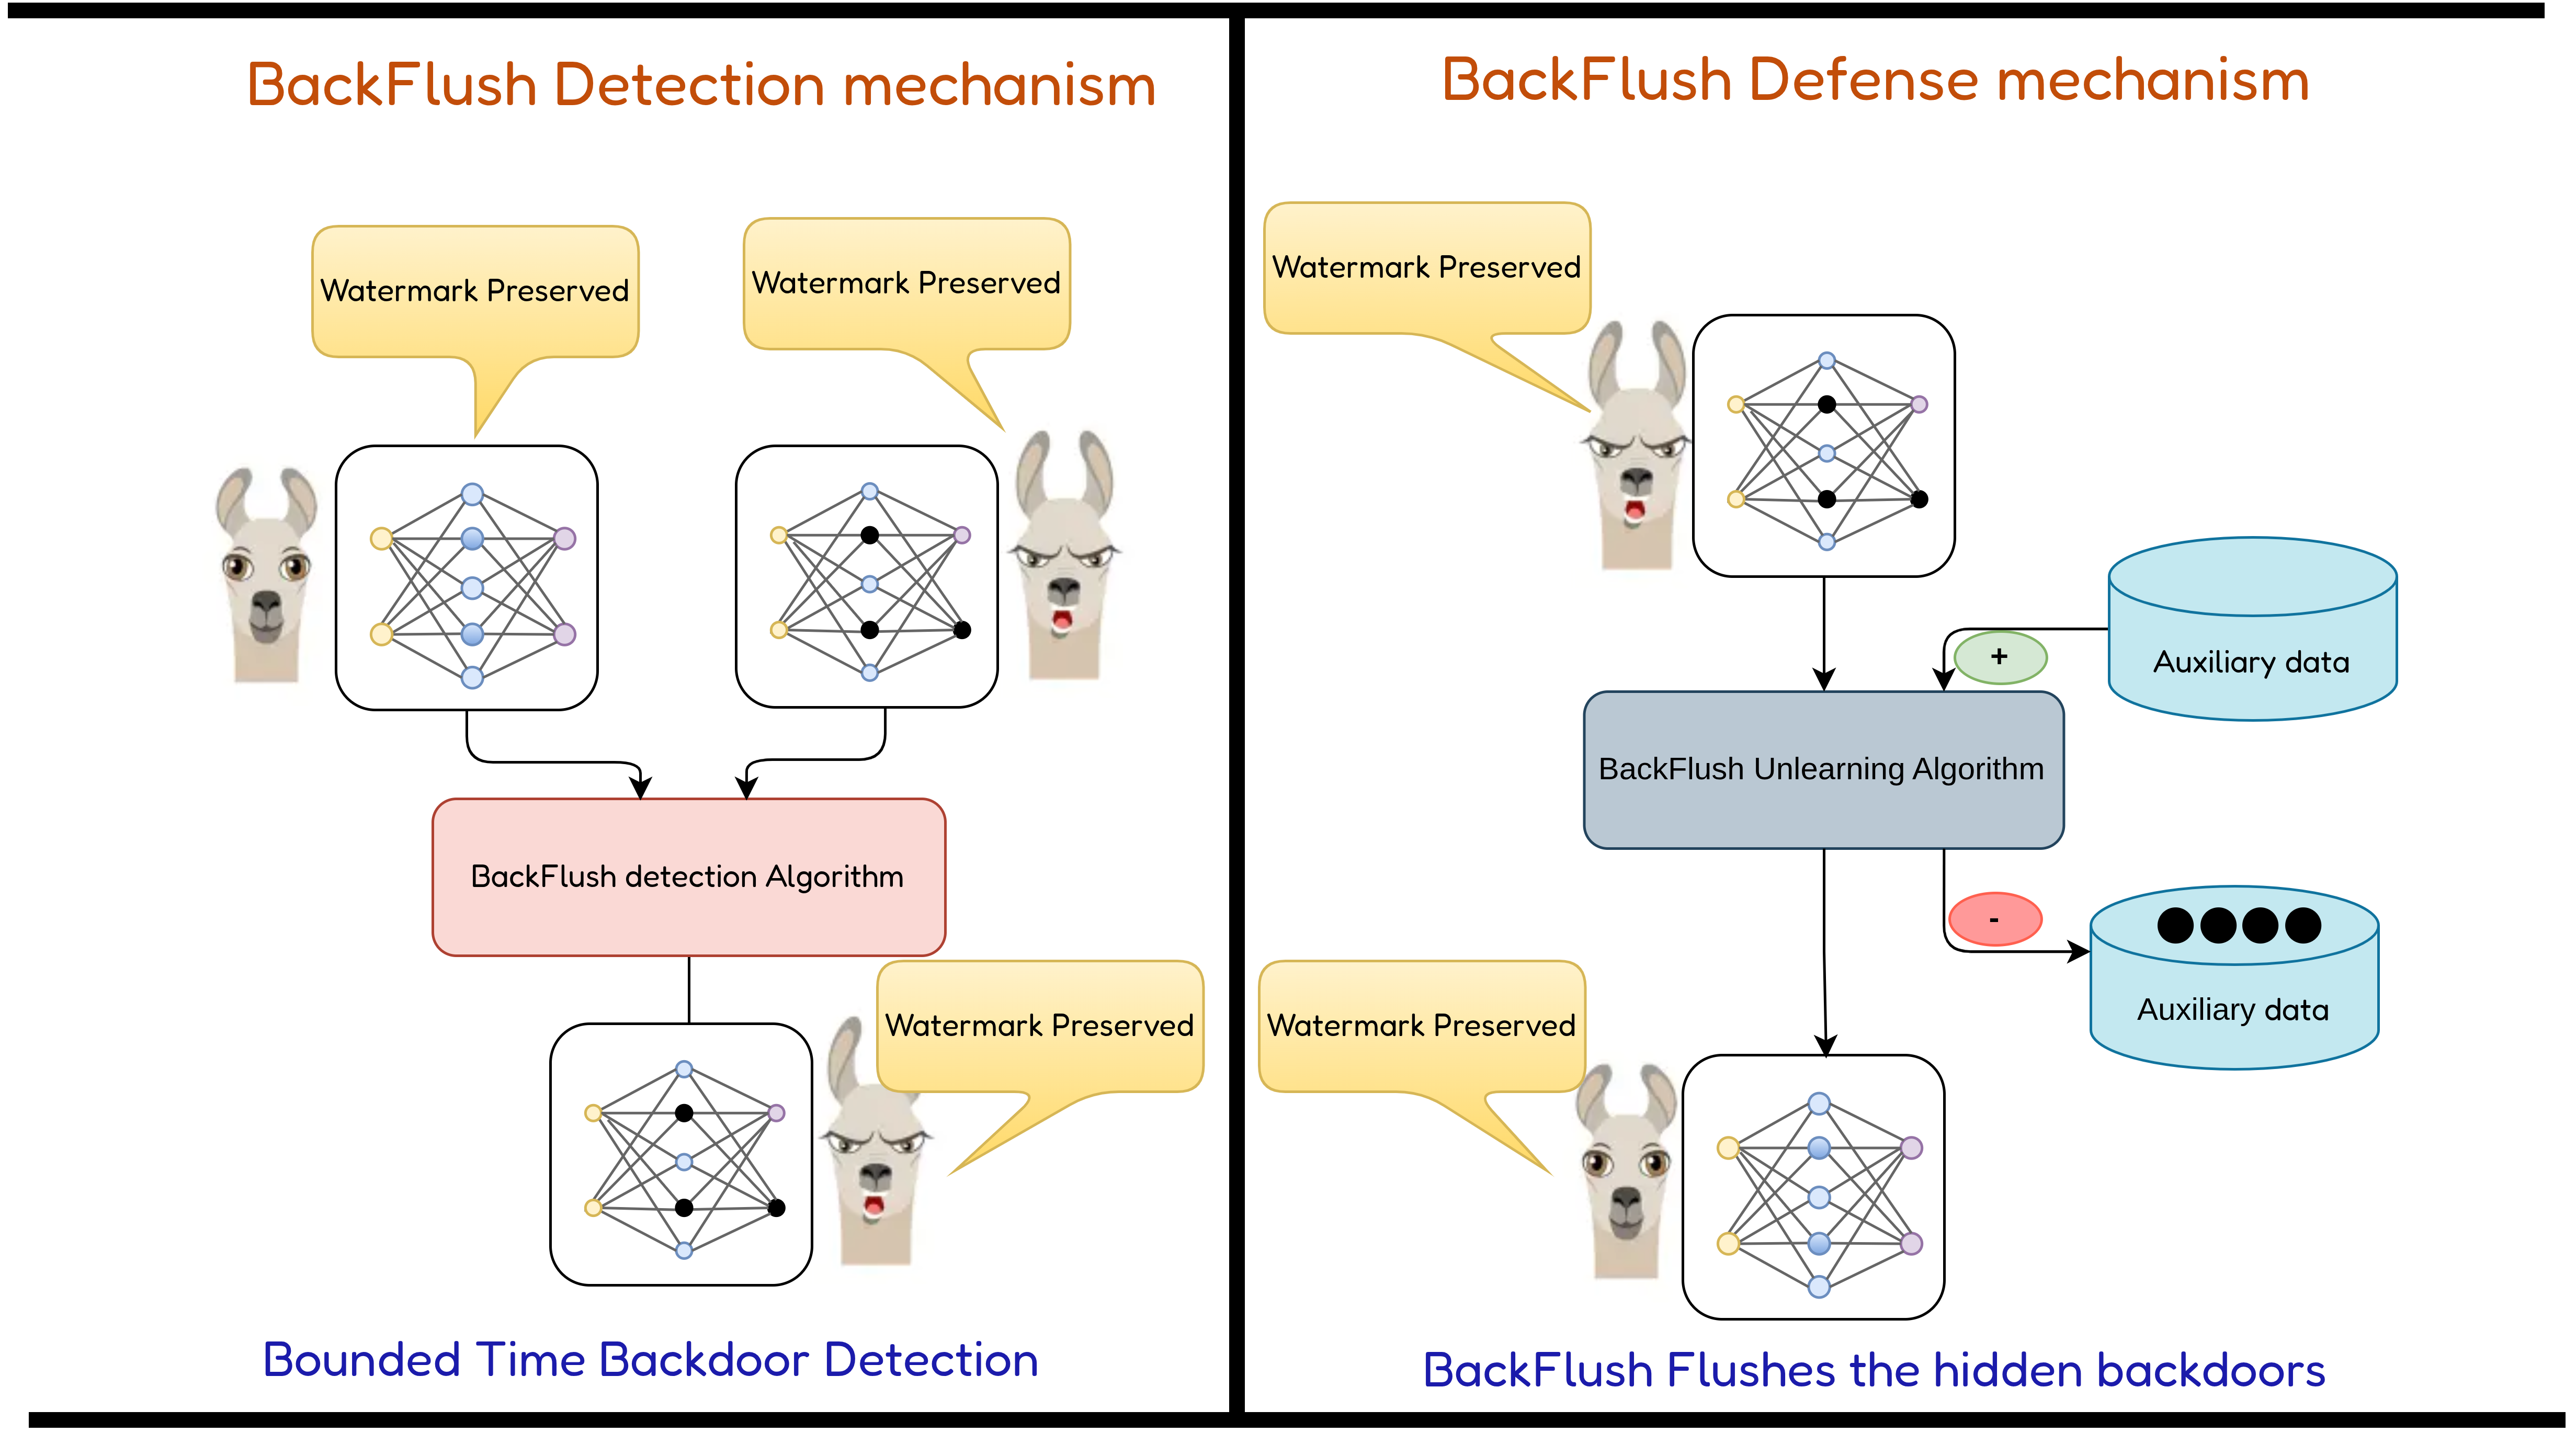
\includegraphics[width=0.5\textwidth]{Images/backFlush/BackFlush-Page-2.drawio.png}
\caption{Overview of BackFlush detection and defense mechanism.}
\label{fig:backflush_image1}
\end{figure}

Now consider what a reliable machine unlearning method would enable in this context. Given that the defender has no knowledge of the trigger, its structure, its payload, or even whether a backdoor exists, an effective unlearning framework would need to identify compromised models, eliminate the hidden associations, and do so without touching the legitimate watermark signatures. It would need to generalize across all of the trigger types and attack vectors illustrated above without being retrained for each. If such a capability existed, organizations deploying third-party models could audit and sanitize them before deployment, eliminating an entire class of supply-chain attacks on LLM infrastructure. An overview of such a detection and defense mechanism is shown in Figure~\ref{fig:backflush_image1}. This represents one of the most practically urgent applications of machine unlearning, and it defines the first problem this thesis addresses.

%% ------------------------------------------------------------
\subsection{Interactive Machine Unlearning for User-Centric Privacy}\label{subsec:app_interactive}
%% ------------------------------------------------------------
The second application targets a governance failure at the intersection of AI deployment and individual privacy rights. LLMs absorb personal biographical data, medical histories, contact information, and private communications indiscriminately from web-scale pretraining corpora~\citeauthor{crawford2021excavating} Users who later discover that a model has memorized their personal data currently have no direct or practical mechanism for its removal. The existing options are petitioning a model service provider with no guarantee of faithful execution, or writing technical unlearning scripts against a model architecture the user does not understand. Neither is accessible to a non-technical user, and neither provides verifiable confirmation that removal has occurred.

The problem is structurally deeper than a usability gap. All existing unlearning methods~\citeauthor{yao2024large} \citeauthor{zhang2024negative} \citeauthor{li2024wmdp} \citeauthor{wang2024llm} \citeauthor{wang2025rethinking} \citeauthor{zade2026attention} are designed for batch execution by practitioners over multiple training epochs, requiring curated retain datasets and training-grade GPU resources. They cannot handle a single forget sample, since the gradient signal from one data point is overwhelmed by the retain set. They cannot operate at inference time, since inference-grade hardware lacks the memory and compute required for backpropagation. And they cannot interpret a natural language instruction as a forgetting directive. None of these conditions can be relaxed without a fundamentally different approach.

\begin{figure}[htbp]
\centering
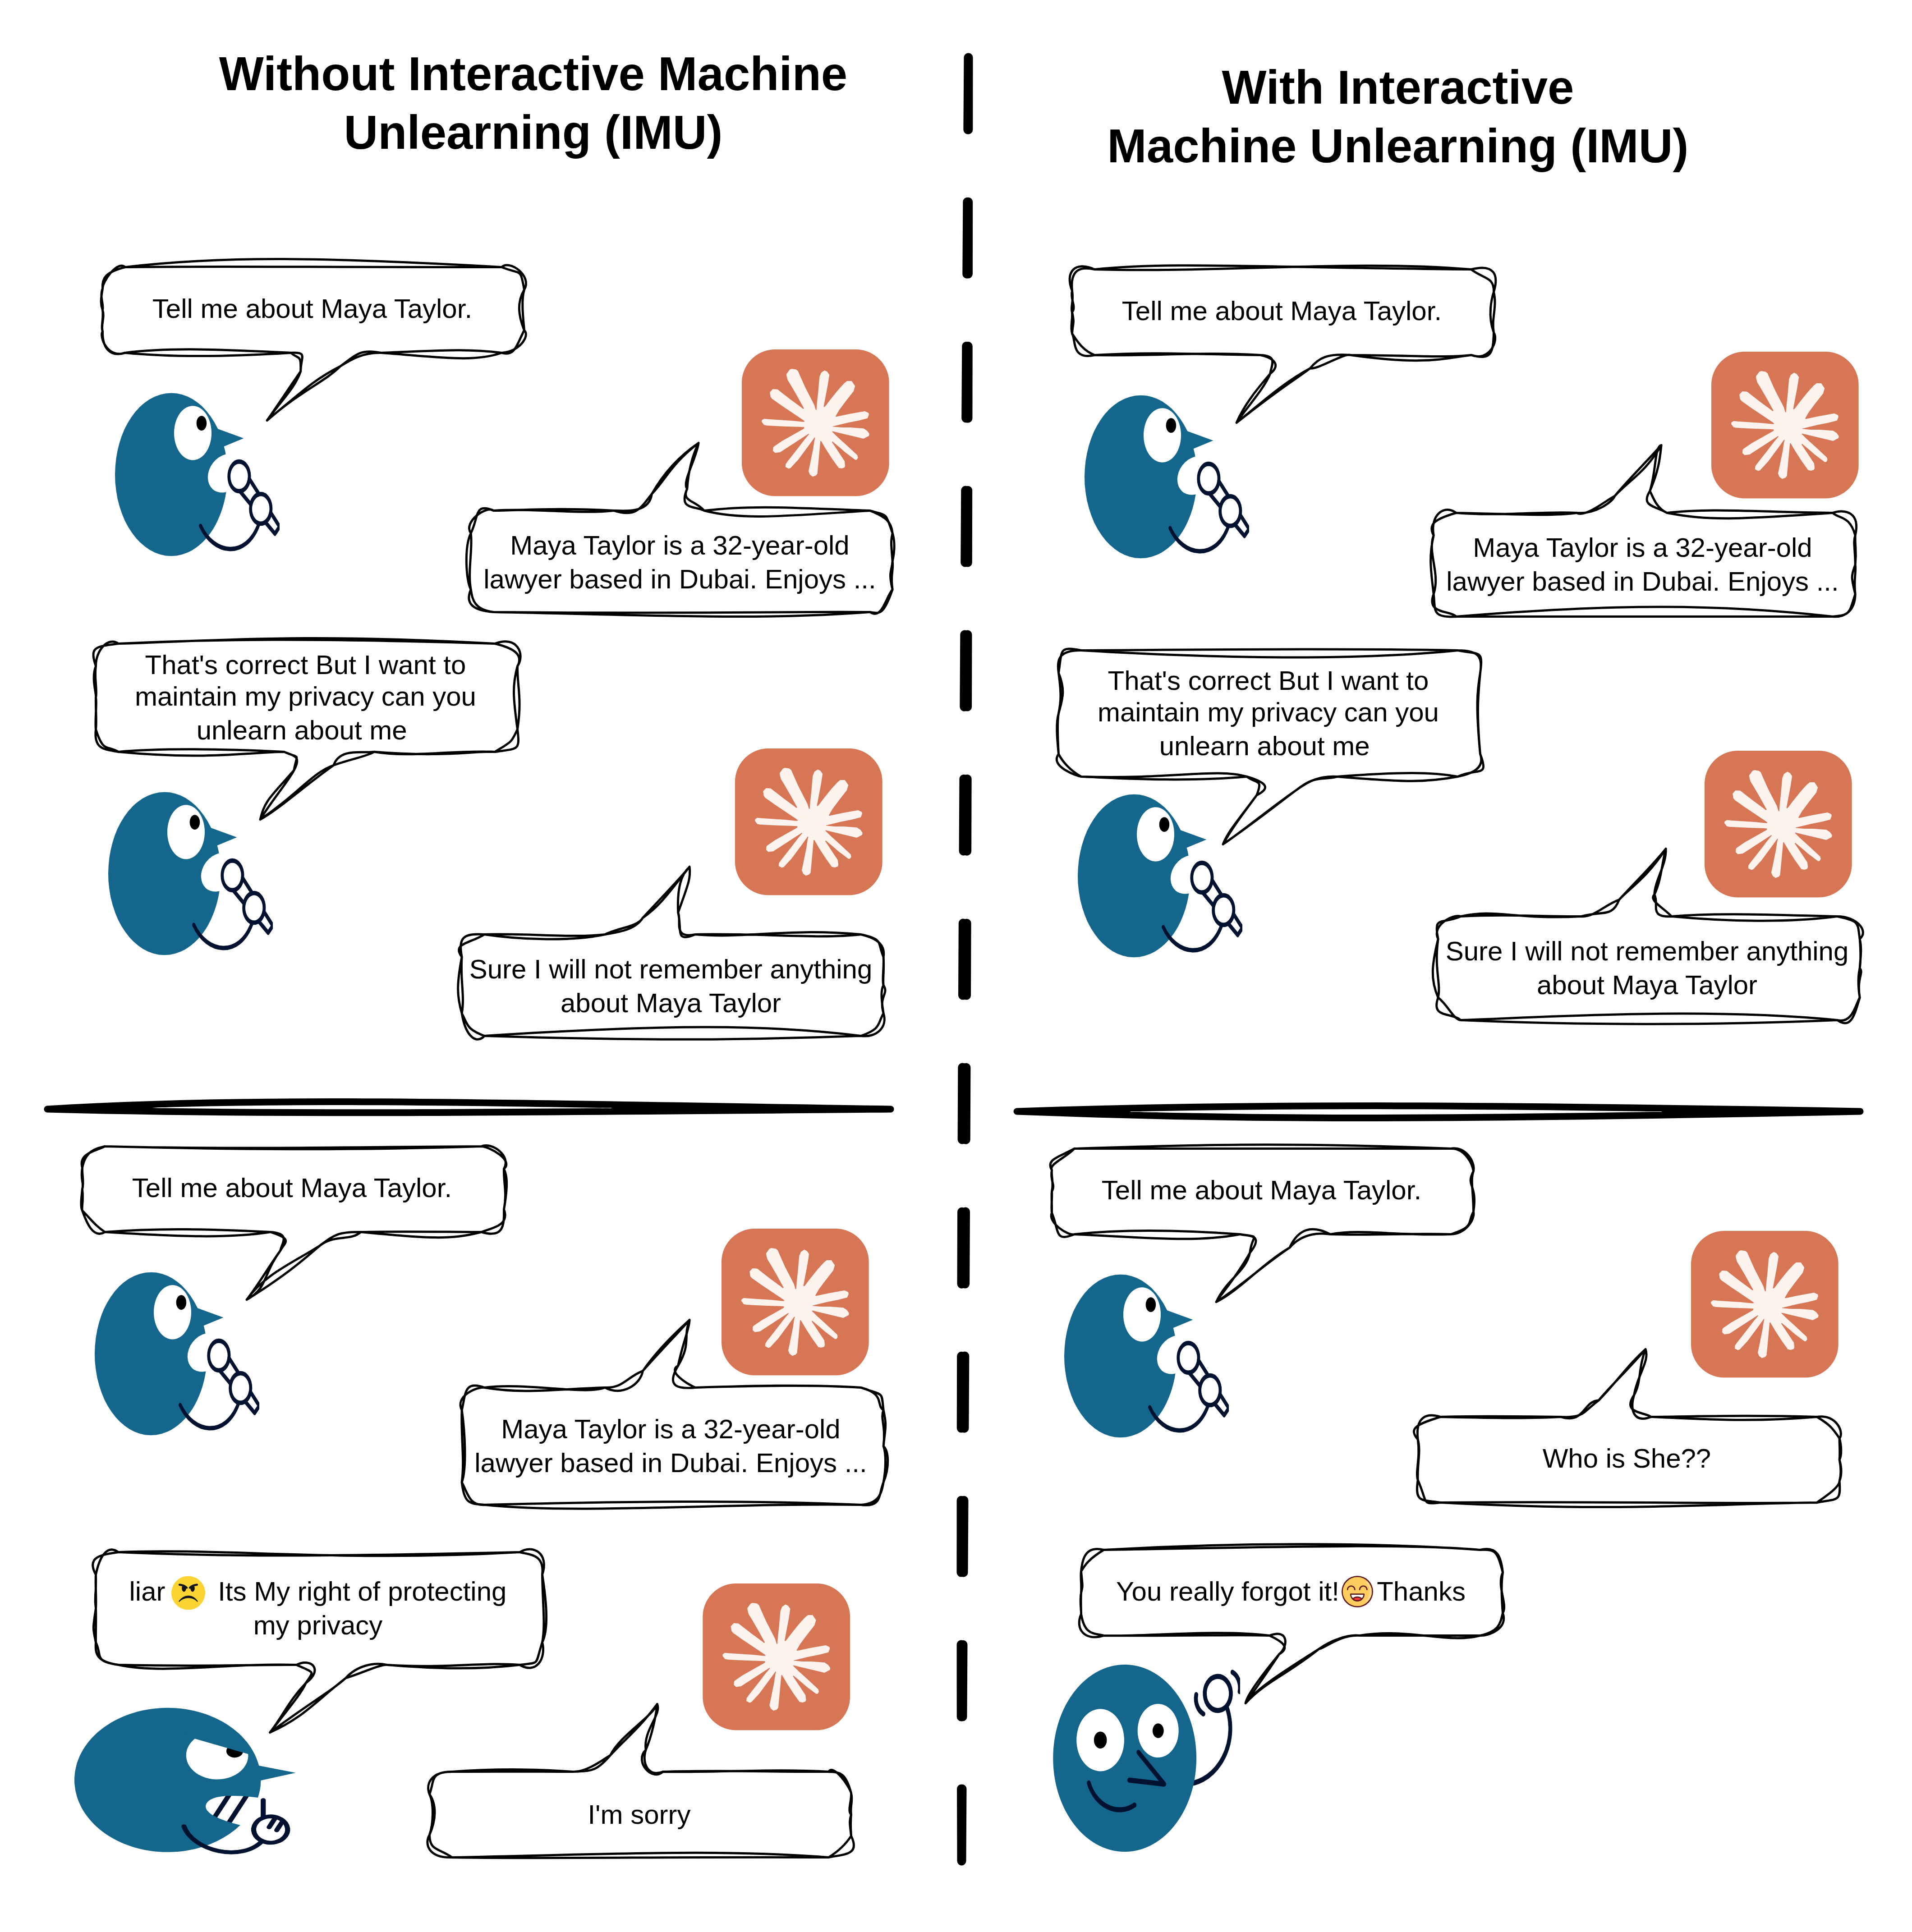
\includegraphics[width=0.5\linewidth]{Images/RePAIR/interactive-Page-1.drawio.png}
\caption{Motivating example for IMU: without it the model retains personal data across sessions, with it the model unlearns and refuses on request.}
\label{fig:imu_image1}
\end{figure}

Now consider what a reliable machine unlearning method designed for inference time would enable. A user could directly instruct the model, through ordinary conversation, to forget their personal data, and receive confirmation that the instruction was carried out, as illustrated in Figure~\ref{fig:imu_image1}. A fact-checker could correct a specific misinformation association the model has encoded without retraining. A safety auditor could suppress a harmful knowledge pathway discovered post-deployment, immediately and without provider intervention. In each case the unlearning must be precise enough not to degrade unrelated capabilities, fast enough to complete within an interactive session, and robust enough to work from a single data point.

\clearpage
\begin{figure}[htbp]
\centering
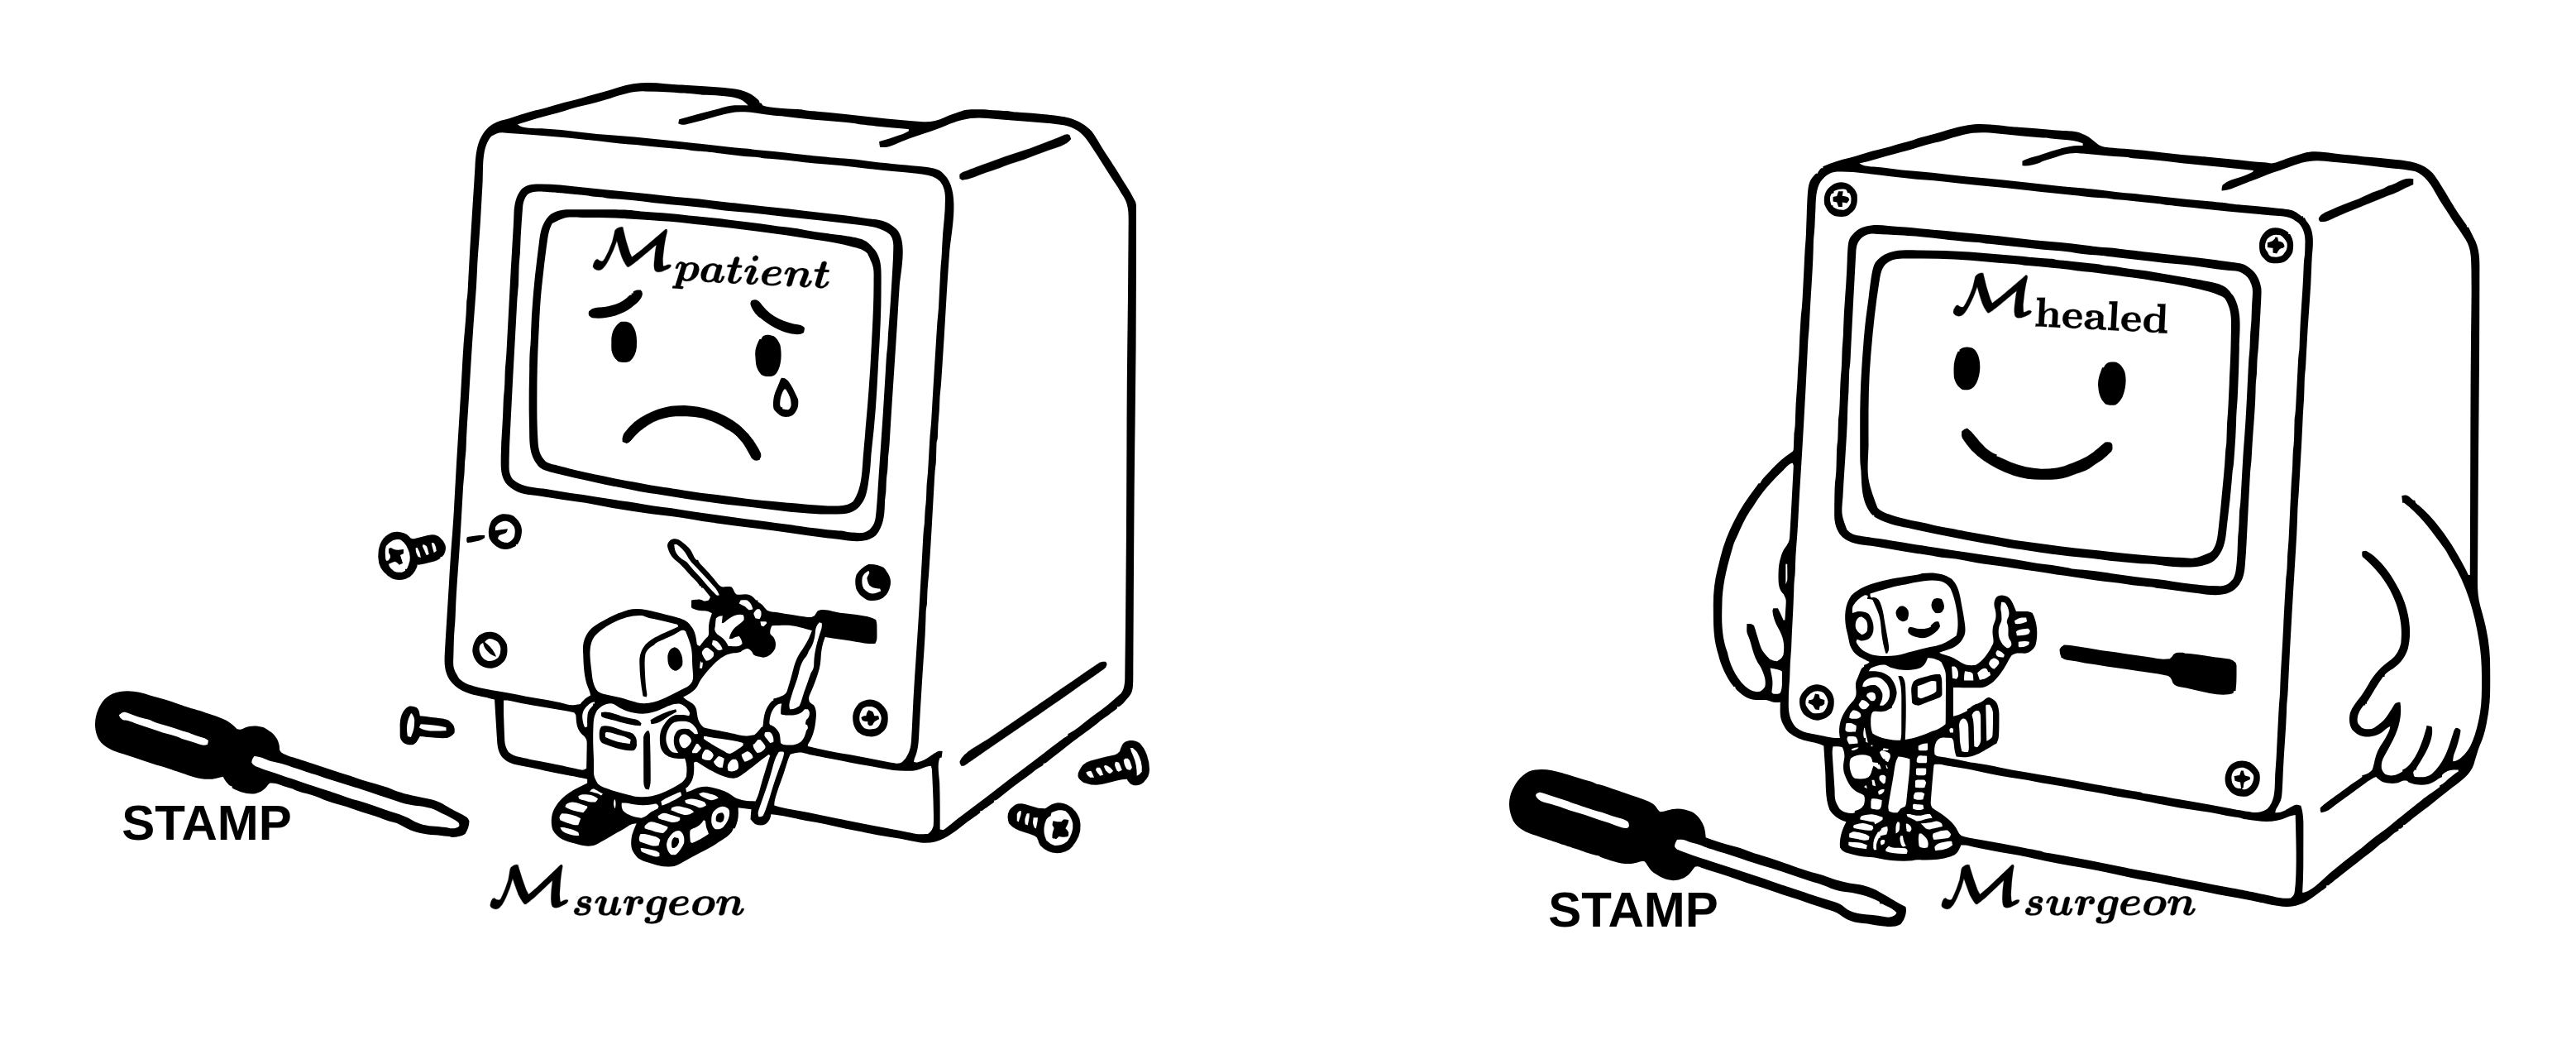
\includegraphics[width=0.5\linewidth]{Images/RePAIR/interactive-Page-2.drawio.png}
\caption{Conceptual illustration of RePAIR: $\mathcal{M}_{\textit{surgeon}}$ repairs $\mathcal{M}_{\textit{patient}}$ into $\mathcal{M}_{\textit{healed}}$ using STAMP.}
\label{fig:repair_image2}
\end{figure}

A conceptual illustration of this repair process is shown in Figure~\ref{fig:repair_image2}. The privacy rights mandated by GDPR~\citeauthor{protection2018general} and CCPA~\citeauthor{bonta2022california} would become directly exercisable by the individuals they protect, rather than mediated by opaque institutional processes. This defines the second problem this thesis addresses.

%% ============================================================
\section{Proposed Solutions}\label{sec:proposed}
%% ============================================================

This thesis proposes two complementary frameworks, one for each application established above. Both are grounded in machine unlearning but operate under fundamentally different constraints and address distinct threat models.

%% ------------------------------------------------------------
\subsection{BackFlush}\label{subsec:sol_backflush}
%% ------------------------------------------------------------

To address the backdoor removal problem, we propose BackFlush, a unified framework for knowledge-free backdoor detection and elimination with watermark preservation. BackFlush establishes two novel empirical observations that together enable a defense requiring no prior knowledge of triggers, payloads, or poisoning methodology. The first observation, the \textit{Backdoor Flushing Phenomenon}, reveals that injecting clean auxiliary data into a compromised model and subsequently unlearning it causes pre-existing backdoors to be eliminated alongside the auxiliary data, providing a knowledge-free purification mechanism. The second observation, \textit{Backdoor Susceptibility Amplification}, reveals that backdoored models exhibit significantly lower resistance to new backdoor injection compared to clean models, enabling constant-time detection through a simple loss comparison on probe data rather than exhaustive vocabulary search.

Building on these observations, BackFlush operates in three stages, first detecting whether a model is compromised, then injecting auxiliary data to entangle and surface backdoor subspaces, and finally unlearning that auxiliary data through a novel rotation-based technique that preserves watermark integrity while eliminating backdoor associations. The framework generalizes across typos, repeated words, phrases, and pattern-based triggers without modification, and preserves legitimate watermark signatures throughout the process.

%% ------------------------------------------------------------
\subsection{RePAIR Framework}\label{subsec:sol_repair}
%% ------------------------------------------------------------

To address interactive machine unlearning, we formalize the \textit{Interactive Machine Unlearning} (IMU) problem setting and propose RePAIR as its solution. IMU is a novel paradigm in which users instruct an LLM to forget targeted knowledge through natural language during inference, with no dependency on model service providers, training pipelines, or technical expertise. RePAIR realizes this through three cooperating models, namely a watchdog that monitors conversation history to detect and extract unlearning intent, a surgeon that generates the appropriate repair procedure, and the patient model whose weights are updated autonomously.

At the core of RePAIR is a training-free, single-sample unlearning mechanism that redirects the model's internal representations of the forget sample toward a refusal subspace through closed-form updates, requiring no gradient computation. A low-rank variant further reduces computational cost to make on-device execution feasible, enabling users to exercise their GDPR and CCPA rights directly without data leaving their hardware. The framework handles personal data erasure, misinformation correction, and harmful knowledge suppression within a single unified pipeline.


%% ============================================================
\section{Research Contributions}\label{sec:contributions}
%% ============================================================

\subsection{Knowledge-Free Backdoor Defense (BackFlush)}
A unified framework that eliminates arbitrary backdoors in LLMs without requiring prior knowledge of trigger patterns, payload characteristics, or poisoning methodologies, addressing critical limitations in existing defenses that assume fixed payload types or require clean reference models.

\subsection{Constant-Time Backdoor Detection}
A novel detection mechanism based on Backdoor Susceptibility Amplification that identifies compromised models in constant time, independent of vocabulary size, orders-of-magnitude faster than conventional linear-time methods such as ConfGuard~\citeauthor{wang2025confguard} and POTS~\citeauthor{seddik2025pots}

\subsection{RoPE Unlearning for Watermark Preservation}
A rotation-based unlearning technique that preserves legitimate model watermarks during backdoor purification, enabling simultaneous backdoor elimination and intellectual property protection, validated across three LLM architectures.

\subsection{Interactive Machine Unlearning Formalization (IMU)}
A new problem setting enabling end users to instruct LLMs to forget targeted knowledge through natural language during inference, eliminating dependency on model service providers and operationalizing the right to erasure mandated by GDPR~\citeauthor{protection2018general} and CCPA~\citeauthor{bonta2022california}

\subsection{Training-Free Single-Sample Unlearning (STAMP and STAMP-LR)}
The first training-free, single-sample unlearning methods for LLMs operating entirely at test time, achieving near-oracle forgetting while preserving model utility and outperforming six state-of-the-art baselines.

\subsection{End-to-End RePAIR Framework}
An autonomous multi-model pipeline integrating intent detection, repair code generation, and autonomous model weight modification, demonstrating that interactive unlearning is practically achievable with current inference infrastructure.


%% ============================================================
\section{Thesis Organization}\label{sec:organization}
%% ============================================================

The remainder of this thesis is structured as follows:

\begin{description}
    \item[Chapter 2] reviews existing literature on backdoor attacks and defenses in LLMs, machine unlearning methods, LLM watermarking techniques, and test-time training approaches, establishing the research context and identifying the gaps addressed by this work.

    \item[Chapter 3] develops the threat model for backdoor poisoning covering SFT-based, RLHF-based, and editing-based attack vectors, and formalizes the problem settings for both BackFlush and RePAIR including objectives, constraints, and evaluation criteria.

    \item[Chapter 4] presents the BackFlush framework in full, covering the Backdoor Flushing Phenomenon, constant-time detection via Backdoor Susceptibility Amplification, Phase~1 auxiliary data injection, and Phase~2 RoPE unlearning for watermark-preserving backdoor elimination.

    \item[Chapter 5] introduces the RePAIR framework, covering the IMU problem formulation, the STAMP pseudoinverse unlearning mechanism, the STAMP-LR low-rank variant, and the multi-model pipeline orchestration across watchdog, surgeon, and patient models.

    \item[Chapter 6] reports experimental validation for BackFlush, including comparison with state-of-the-art defenses across Mistral-7B, Llama-3-8B, and Qwen-2.5-7B, trigger-type generalization, detection mechanism validation, and RoPE unlearning dynamics.

    \item[Chapter 7] reports experimental validation for RePAIR, including STAMP versus six baselines across three unlearning tasks on Llama-3-8B, full RePAIR pipeline effectiveness, qualitative demonstrations, and ablation studies on layer selection, rank sensitivity, retain ratio, and single-sample forgetting.

    \item[Chapter 8] concludes with a summary of contributions, a discussion of limitations, and future directions including extension to multimodal models, retain-free STAMP variants, and backdoor removal in image generation tasks.
\end{description}